\documentclass[12pt, twocolumn]{article}
\usepackage{amsmath}
\usepackage{amsfonts}
\usepackage{graphicx}
\usepackage{mathtools}
\usepackage{fullpage}
\usepackage{float}
\usepackage{color, soul}

\begin{document}
\title{ 6.867 Term Project: \\ An Exploration of Deep Learning and \\ Convolutional Neural Nets for Image Classification\\ }
 \author{Kathryn Evans, Andres Hasfura and Remy Mock}
\maketitle

\section{ Introduction} 
Neural networks are a useful machine learning framework that's primary benefit is that instead of specifying the basis functions relating input to output,  more or less learns the connectivity, since the optimal basis functions could be complicated and non-intuitive, such as in the case of images. Such an approach is Artificial Neural Networks (ANN). The idea of a neural network replaces the known basis functions with features, which are parametric functions of activations, learned from the input data in the first layer of learning, and then utilize a second layer to learn the relationship of the output data from those selected features.

Through this course, a simple singular layer artificial neural network was presented. However, much like the neural networks in the human brain visual system which provided the inspiration for artificial neural networks, the architecture used for machine learning neural networks can be more complicated and complex than a single hidden layer. The idea of utilizing many layers is known as deep learning.  Increasing layers, while drastically more parameters and computation,  allows for more complex input/output relationship and an ability to classify based on both information from low and high level features.

Deep learning, although not a recent idea, has recently exploded in popularity due to rise in labeled data and general purpose GPU programming and is revolutionizing very important subfields within artificial intelligence. Machine learning, machine vision, and natural language processing are examples of area in which the use of deep learning has produced large jumps in performance on difficult test sets. Deep nets are now being used anywhere from pedestrian detection for autonomous vehicles \cite{Szarvas2006}, to facial expression recognition \cite{Li2015} to classifying whether or not a selfie is good \cite{Karpathy}. 
	
Not only do deep nets contain more hidden layers but a multitude of different types of layers. Each layer type has different connectivity and objectives allowing for a greater richness of information. For use with images convolutional layers are especially beneficial for examining only the relevance of spatially nearby pixels in the context of determining features. Arrangements of convolutional layers as well as other types of layers leads to Convolutional Neural Networks (CNN). 

In this project, we want to explore the benefits of deep nets as well as convolutional neural networks for image classification.  Our goal is to generalize the benefit on image classification performance of firstly, additional fully connected hidden layers and secondly, more complicated convolutional layers and architectures. Not only do we want to gain familiarity with concept and tools used in deep learning but we also hope to document generalities by applying these approaches to multiple image datasets. The generalities we hope to explore include the following: How does the number of layers effect the amount of training data needed? How to choose architectures? 

\section{Approach and Methodology}
	
In this project, we seek to implement a version of multilayer neural nets for supervised learning on specifically images. We plan on trying our implementations on datasets of varying difficulty, starting from MNIST, so that we do not have to worry about data generation and labeling and provide generalization about the neural net choices. Because we are specifically interested in applying our implementation to images we hope to see benefit of making the network out of convolution layers, where not all nodes are connected and we will compare this to a implementation with fully connected layers.

 We will then compare our rudimentary approach to a professional library for deep learning, specifically TensorFlow. Obviously the professional library will allow for better results and more interesting conclusions but building and implementing a simplified version will give a better understanding into how the neural network works. 

\subsection{Neural Network Basics}


\begin{figure}
\includegraphics[scale=.7]{simpleNN.png}

\caption{Visualization of a simple Neural Network with 1 hidden layer \cite{Bishop} . }
\label{fig:basicNN}
\end{figure}





\subsection{Multi-layer Neural Network}
For forward propagation is straight forward, you simply continue the formula for a single hidden layer and chain them together for more layers. 

For backwards propagation the error for each fully connected layer, $l$ is computed from the error of its output layer, $l+1$  

\begin{equation}
\delta^{(l)}=((W^{(l)})^T \delta^{(l+1)}) \cdot f ^{\prime} (z^{(l)})
\end{equation}

and the following derivatives 
\begin{equation}
\nabla_{W^{(l)}}J(W,b;x,y) = \delta^{(l+1)}(a^{(l)})^T
\end{equation}
\begin{equation}
\nabla_{b^{(l)}}J(W,b;x,y)= \delta^{(l+1)}
\end{equation}

As the network grows bigger and bigger the computational time becomes more and more of a constraint. So for all studied neural  networks we will used Stochastic Gradient descent as opposed to batch methods. We simply halve the learning rate after each epoch. As mentioned in Stochastic Gradient Descent, we also randomly shuffle the data before each epoch, which tends to provide better convergence.


\subsection{General Architecture of a Convolutional Neural Network}
As opposed to a simple neural network, a convolutional neural network is specifically designed to take advantage of the 2-d structure of an input image by considering only local connections and tied weights followed by some form of pooling which results in translation invariant features. Compared to regular neural nets,  CNNs  have many fewer parameters than networks of similar size and thus they are easier to train.



\subsubsection{Convolutional Layer}
The idea of the CNN is to no longer have fully connected layers. Instead not every node is connected to every other node. Instead these relationships are described by a kernel. Of particular interest in the convolutional kernel. But instead of hard coding the filters, the filters used are learned by training. 

By sub sampling the image and having learned features over smaller segments of the larger image. The feature detector learning from the subsection can then be applied anywhere in the remaining image. Specifically, we can take the learned subsection features and convolve them with the larger image there by  transforming the 2-D images into a 3-D space. For a  $M * N $ size image, using $K$ filters that are $m * n$,  after convolution, there are  $ K * (M - m + 1) * (N - n + 1) $ sub images. Using this method, we decrease the size of each image, but at the same time we learn low level features. 


Generally, the process that occurs in a convolution layer can be described as for each image, $x_n$ for $n=1..N$ and for each filter $k=1...K$ in the convolution layer, $c$
\begin{equation}
a_{n,k}^{(c)}= x_n \ast w_k^{(c)} + b_k^{(c)}
\end{equation}
\begin{equation}
f_{n,k}= \tilde{g}(a_{n,k}^{(c)})
\end{equation}
 
 Where $\ast$ is the convolution operator. 
 
 Layers closer to the input have fewer filters than those layers further up the chain due t . The number of feature maps directly controls capacity and so that depends on the number of available examples and the complexity of the task. The trick is thus to find the right level of ?granularity? (i.e. filter shapes) in order to create abstractions at the proper scale, given a particular dataset

Also CNNs introduce the idea of tied weights, which mean that certain connections between one layer to the next are defined to be the same which dramatically reduces the number of parameters needed to describe and set up the network. This idea is shown in fig. \ref{fig:conv}.



\begin{figure}
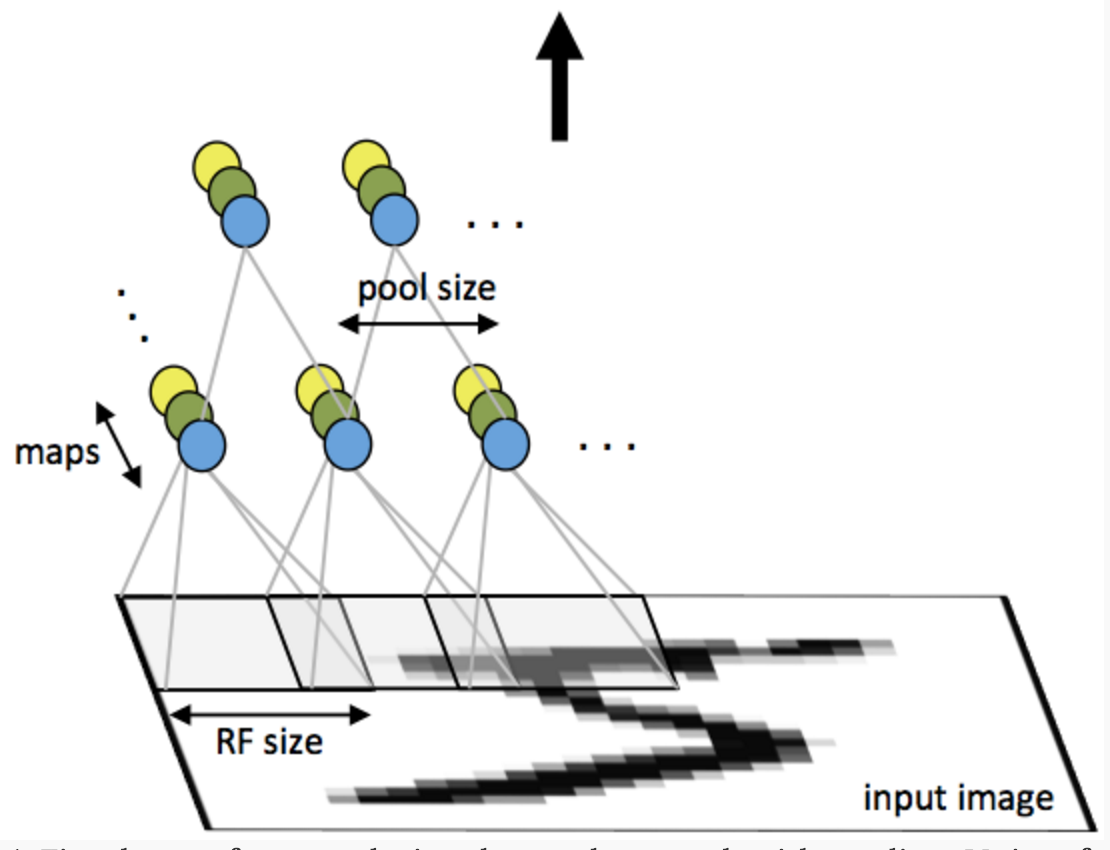
\includegraphics[scale=.4]{convgraphic.png}

\caption{Layer of a convolutional neural network with pooling. Nodes of the same color have tied weights and units of different color represent different filter maps \cite{StanfordTut}. }
\label{fig:conv}
\end{figure}


\subsubsection{Pooling Layer}
The features learned using convolution, are next used for classification. Previously with the fully connected neural network we utilized a softmax classifier, but this can be computationally challenging and expensive. Instead, pooling layers take advantage of a single parameter of these features, such as the mean, ( 'mean pooling') or max ( 'max pooling'), at  various regions in the image. Not only does this reduce the dimensionality of the result but can also help reduce over-fitting.

The region to be pooled over is determined by the pooling dimensions. It again involves a convolution, this time between regions specified by the pooling dimensions and the results from the previous convolution layer. 



\subsection{Backprop for CNN}
Derivatives are needed . Up sample
\subsection{Professional Libraries}
\subsubsection{TensorFlow}



\subsection{Datasets Considered}



\section{Results}



\subsection{Benchmarking with MNIST}
\begin{center}
\begin{table*}[t]
\begin{tabular} { |c | c | c | c | }
    \hline
    NN Type & LeCun Error  &  Our Error  & Tensor Flow Error \\ \hline
    2-layer NN, 300 hidden units, mean square error & 4.7 &  & \\ \hline
    2-layer NN, 1000 hidden units & 4.5 & & \\ \hline
    3-layer NN, 300+100 hidden units & 3.05 & &  \\ \hline
    3-layer NN, 500+150 hidden units & 2.95 & & \\ \hline
    Convolutional net LeNet-1 & 1.7 &  & \\ \hline 
    Convolutional net LeNet-4 & 1.1& & \\ \hline 
    Convolutional net LeNet-5 &  0.95 & &\\ \hline
\end{tabular}
\label{table: MNISTLeCun}
\caption{Comparison of Test Error results for multilayer ANN and CNN with published results \cite{LeCun1998}.}
\end{table*}
\end{center}



The MNIST is a well-known dataset of handwritten digits, 0-9, comprising 60,000 training examples and 10,000 test examples \cite{MNIST}  that can be used for image classification.  This data set arose from the U.S. Postal Service zip code database in order to help the scanning and transport of package to the right area. The images are all centered in 28 x 28.

\begin{figure}
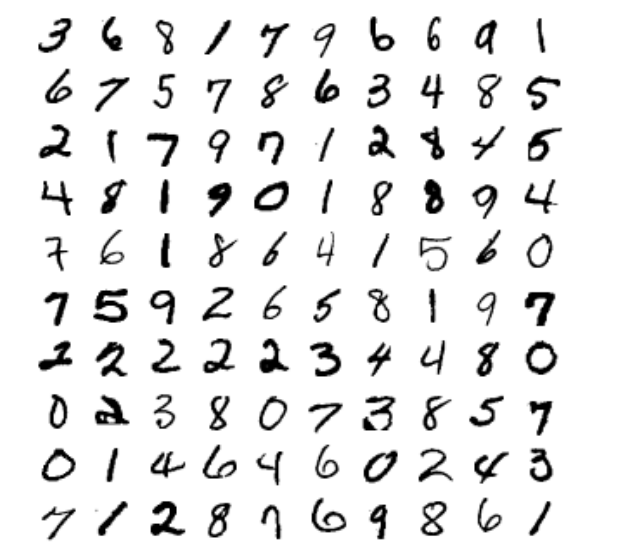
\includegraphics[scale=.8]{MNISTnos.png}
\label{fig:MNISTex}
\caption{Sample entries of the MNIST dataset \cite{LeCun1998}}
\end{figure}

Already done and thoroughly explored by many people included Yann LeCun \cite{LeCun1998} however it provides a good system to check our results by since it is so well documented.  Replication of the architects of both the fully-connected and convolutional neural nets provided in this paper is the first objective of our study. By comparing our results  for different layers and types of layers to published and documented results, we can make sure our implementation is working before taking on a more complicated dataset. 


 We specifically chose to replicate the 2 and 3 layer fully connected neural nets as well as LeNet-1 and LeNet-5 with no preprocessing or distortions. 

\subsubsection{Replication of NNs}
\subsubsection{Replication of LeNet-1}
\subsubsection{Replication of LeNet-5}
 
\subsection{Other dataset}
\section{Conclusions}

\section{Areas for further work}

\bibliographystyle{unsrt}
\bibliography{references}
 \end{document}
